\documentclass[UTF8]{ctexart}
\usepackage{geometry}
\geometry{a4paper, margin=2.5cm}
\usepackage{graphicx}
\usepackage{listings}
\usepackage{xcolor}
\usepackage{fontspec}
\usepackage{float}
\usepackage{hyperref}
\usepackage{url}
\hypersetup{colorlinks=true, linkcolor=blue, urlcolor=blue}
\graphicspath{{D:/code/LATEX/Conmmunication}}
\setmonofont{DejaVu Sans Mono}  % 若系统无此字体，可改为 Courier New 或 SimHei
\lstset{
    basicstyle=\ttfamily\small,
    breaklines=true,
    frame=single,
    numbers=left,
    numberstyle=\tiny,
    tabsize=4,
    language=C,
    keywordstyle=\color{blue},
    commentstyle=\color{green!60!black},
    stringstyle=\color{red}
}

\title{模拟调制实验}
\author{}

\begin{document}
\maketitle

\begin{center}
    \textbf{班级：}2024217802\quad \textbf{姓名：} 严子竣\quad \textbf{学号：}2024212622
\end{center}

\section{高斯噪声的产生与绘制}

\subsection{AWGN的产生与绘制}

本部分使用低通滤波器从白噪声产生带限高斯噪声，并绘制窄带高斯噪声及其同相分量波形。参数设置中带宽 \(B=100\) Hz，中心频率 \(f_c=2000\) Hz，采样率远高于载频以满足奈奎斯特条件。

代码如下（对应文件AWGN.m）：

\begin{lstlisting}[language = MATLAB]
clear; clc; close all;

%% 参数设置
B = 100;            % 带宽 (Hz)
fc = 2000;          % 中心频率 (Hz)，远大于 B
fs = 25 * fc;          % 采样率 (Hz)，满足 fs >= 2(f_c+B)
T = 0.01;              % 信号时长 (s)
N = round(T * fs);  % 样本点数
t = (0:N-1)/fs;

% 噪声功率谱密度 (假设单位：V^2/Hz)
N0 = 1;             % 单边带功率谱密度
sigma2 = N0 * B;    % 噪声方差

%低通滤波器 (截止频率 B/2)
lpFilt = designfilt('lowpassfir', 'PassbandFrequency', B/2, ...
                     'StopbandFrequency', B/2 + B/5, 'SampleRate', fs);

% 生成独立同相/正交高斯白噪声
n_I = filter(lpFilt, sqrt(sigma2) * randn(N, 1));
n_Q = filter(lpFilt, sqrt(sigma2) * randn(N, 1));

n = n_I .* cos(2*pi*fc*t) - n_Q .* sin(2*pi*fc*t);

figure('Position', [100, 100, 1200, 600]);

subplot(2,1,1);
plot(t, n, 'k', 'LineWidth', 0.8);
xlabel('时间 (s)'); ylabel('幅度'); title('实窄带高斯噪声 n(t)');
grid on; xlim([0, T]);

subplot(2,1,2);
plot(t, n_I, 'b', 'LineWidth', 1);
xlabel('时间 (s)'); ylabel('幅度'); title('同相分量 n_I(t)');
grid on; xlim([0, T]);

\end{lstlisting}

仿真结果：

\begin{figure}[H]
    \centering
    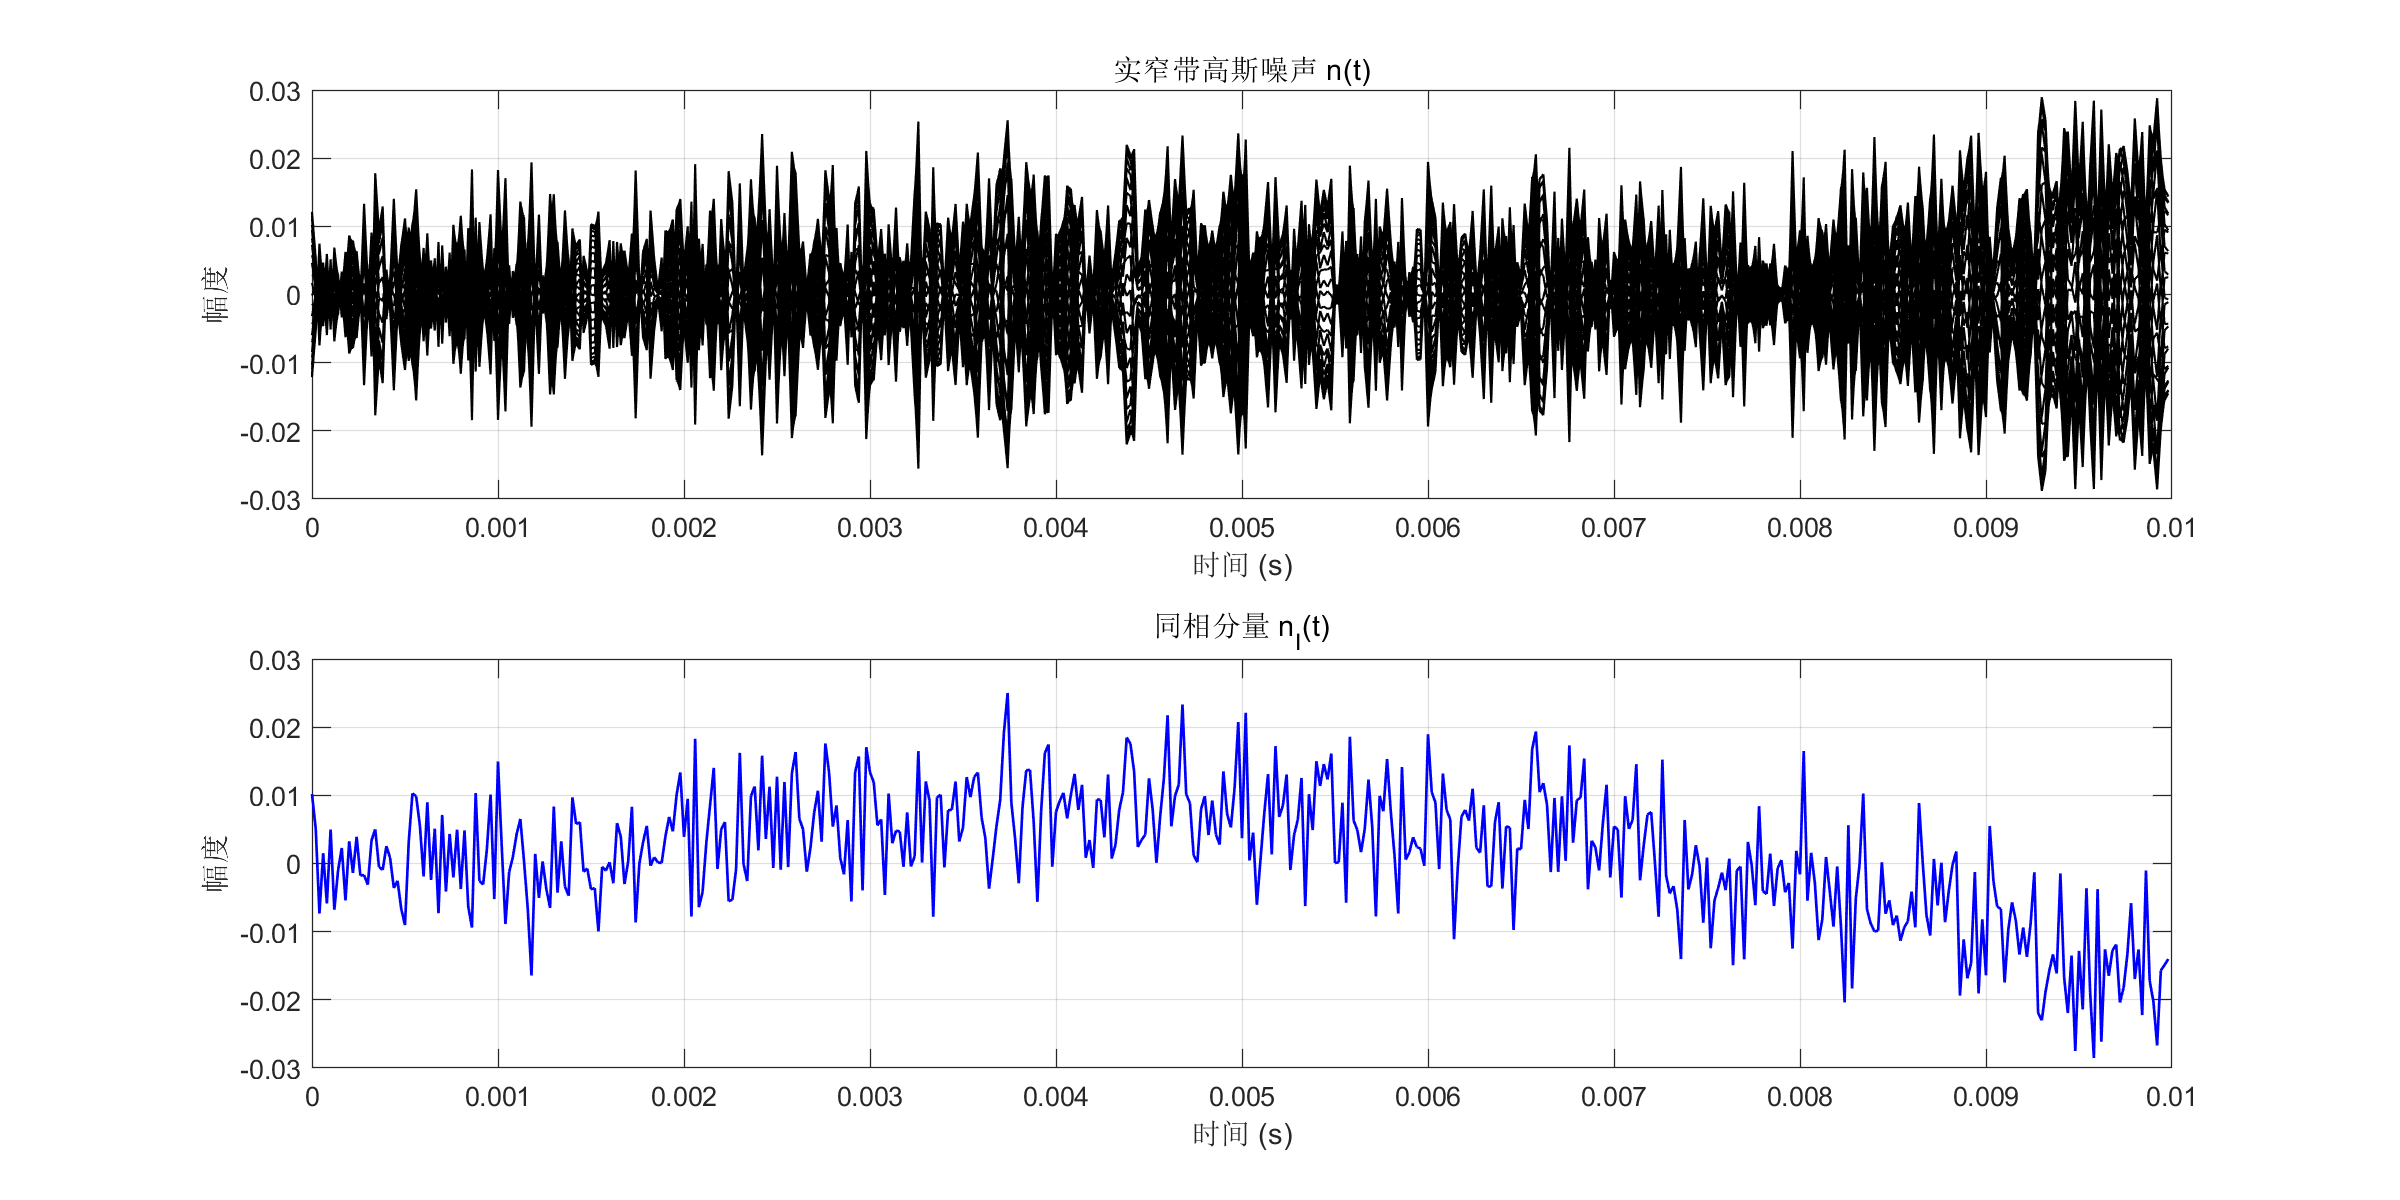
\includegraphics[width=\textwidth]{AWGN.png}
    \caption{加性白高斯噪声及其同相分量}
\end{figure}

\subsection{窄带白高斯噪声的分布与自相关验证}

分别考虑采样率等于带宽和大于带宽两种情况，验证同相分量的高斯分布和自相关特性。对于 \(f_s = B\)，采样点独立；对于 \(f_s > B\)，通过低通滤波产生相关序列。直方图与理论高斯曲线吻合，自相关函数在 \(f_s = B\) 时近似冲激，在 \(f_s > B\) 时符合 \(\mathrm{sinc}(B\tau)\) 函数。

代码如下（对应文件Gauss\_noise.m）：

\begin{lstlisting}[language = MATLAB]
clear; clc; close all;

%% 参数设置
B = 100;            % 带宽 (Hz)
fc = 2000;          % 中心频率 (Hz)，远大于 B
fs1 = B; %基础要求
fs2 = 4 * B; %进阶要求
T = 5;              % 信号时长 (s)

N1 = round(T * fs1);  % 样本点数
N2 = round(T * fs2);

t1 = (0:N1-1)/fs1;
t2 = (0:N2-1)/fs2;

% 噪声功率谱密度 (假设单位：V^2/Hz)
N0 = 1;             % 单边带功率谱密度
sigma2 = N0 * B;    % 噪声方差

n_I_independent = sqrt(sigma2) * randn(N1, 1); %独立高斯序列

figure('Position', [100, 100, 1200, 800]);
%分布验证
subplot(2,2,1);
histogram(n_I_independent, 'Normalization', 'pdf', 'BinWidth', 0.2);
hold on;
x = linspace(-4*sqrt(sigma2), 4*sqrt(sigma2), 200);
pdf_theory = (1/sqrt(2*pi*sigma2)) * exp(-x.^2/(2*sigma2));
plot(x, pdf_theory, 'r-', 'LineWidth', 2);
xlabel('n_I'); ylabel('概率密度'); title('fs = B: 同相分量直方图');
legend('仿真', '理论高斯'); grid on;

%自相关验证
subplot(2,2,2);
max_lag = round(0.1*fs1);   % 观察0.1秒内
[R, lags] = xcorr(n_I_independent, max_lag, 'normalized');
plot(lags/fs1, R, 'b-');
hold on;
stem(0, 1, 'r', 'LineWidth', 2, 'MarkerSize', 8);
xlabel('时延 (s)'); ylabel('归一化自相关'); title('fs = B: 自相关函数');
xlim([-0.1, 0.1]); grid on;
legend('仿真', '理论冲激');
% 正态性检验
[h1, p1] = jbtest(n_I_independent);
fprintf('fs = B: Jarque-Bera 检验 h = %d, p = %.4f\n', h1, p1);
fprintf('实测方差: %.4f, 理论方差: %.4f\n', var(n_I_independent), sigma2);

%低通滤波器 (截止频率 B/2)
lpFilt = designfilt('lowpassfir', 'PassbandFrequency', B/2, ...
                     'StopbandFrequency', B/2 + B/5, 'SampleRate', fs2);

sigma2_in = sigma2 * fs2 / B;   % 输入白噪声方差
white_noise = sqrt(sigma2_in) * randn(N2, 1);
n_I_correlated = filter(lpFilt,white_noise);

% 去除滤波器暂态 (取后半部分)
filter_order = length(lpFilt.Coefficients);
n_I_correlated = n_I_correlated(filter_order:end);
N2_eff = length(n_I_correlated);
t2_eff = (0:N2_eff-1)/fs2;

% 分布验证
subplot(2,2,3);
histogram(n_I_correlated, 'Normalization', 'pdf', 'BinWidth', 0.2);
hold on;
x2 = linspace(-4*sqrt(sigma2), 4*sqrt(sigma2), 200);
pdf_theory2 = (1/sqrt(2*pi*sigma2)) * exp(-x2.^2/(2*sigma2));
plot(x2, pdf_theory2, 'r-', 'LineWidth', 2);
xlabel('n_I'); ylabel('概率密度'); title('fs > B: 同相分量直方图');
legend('仿真', '理论高斯'); grid on;

%自相关验证
subplot(2,2,4);
max_lag_sec = 0.05;         % 观察 50 ms
max_lag_samp = round(max_lag_sec * fs2);
[R_corr, lags_corr] = xcorr(n_I_correlated, max_lag_samp, 'normalized');
lags_time = lags_corr / fs2;
% 理论自相关 (归一化): R_theory(tau) = sinc(B * tau)
tau_theory = linspace(-max_lag_sec, max_lag_sec, 500);
R_theory = sinc(B * tau_theory);

plot(lags_time, R_corr, 'b-', 'LineWidth', 1.5); hold on;
plot(tau_theory, R_theory, 'r--', 'LineWidth', 1.5);
xlabel('时延 \tau (s)'); ylabel('归一化自相关'); title('fs > B: 自相关函数');
legend('仿真', '理论 sinc(B\tau)'); grid on;
xlim([-max_lag_sec, max_lag_sec]);
% 正态性检验
[h2, p2] = jbtest(n_I_correlated);
fprintf('fs > B: Jarque-Bera 检验 h = %d, p = %.4f\n', h2, p2);
fprintf('实测方差: %.4f, 理论方差: %.4f\n', var(n_I_correlated), sigma2);

\end{lstlisting}

命令行输出：
\begin{lstlisting}[language = MATLAB]
fs = B: Jarque-Bera 检验 h = 0, p = 0.5000
实测方差: 100.8026, 理论方差: 100.0000
fs > B: Jarque-Bera 检验 h = 0, p = 0.0888
实测方差: 110.7303, 理论方差: 100.0000
\end{lstlisting}

仿真结果：

\begin{figure}[H]
    \centering
    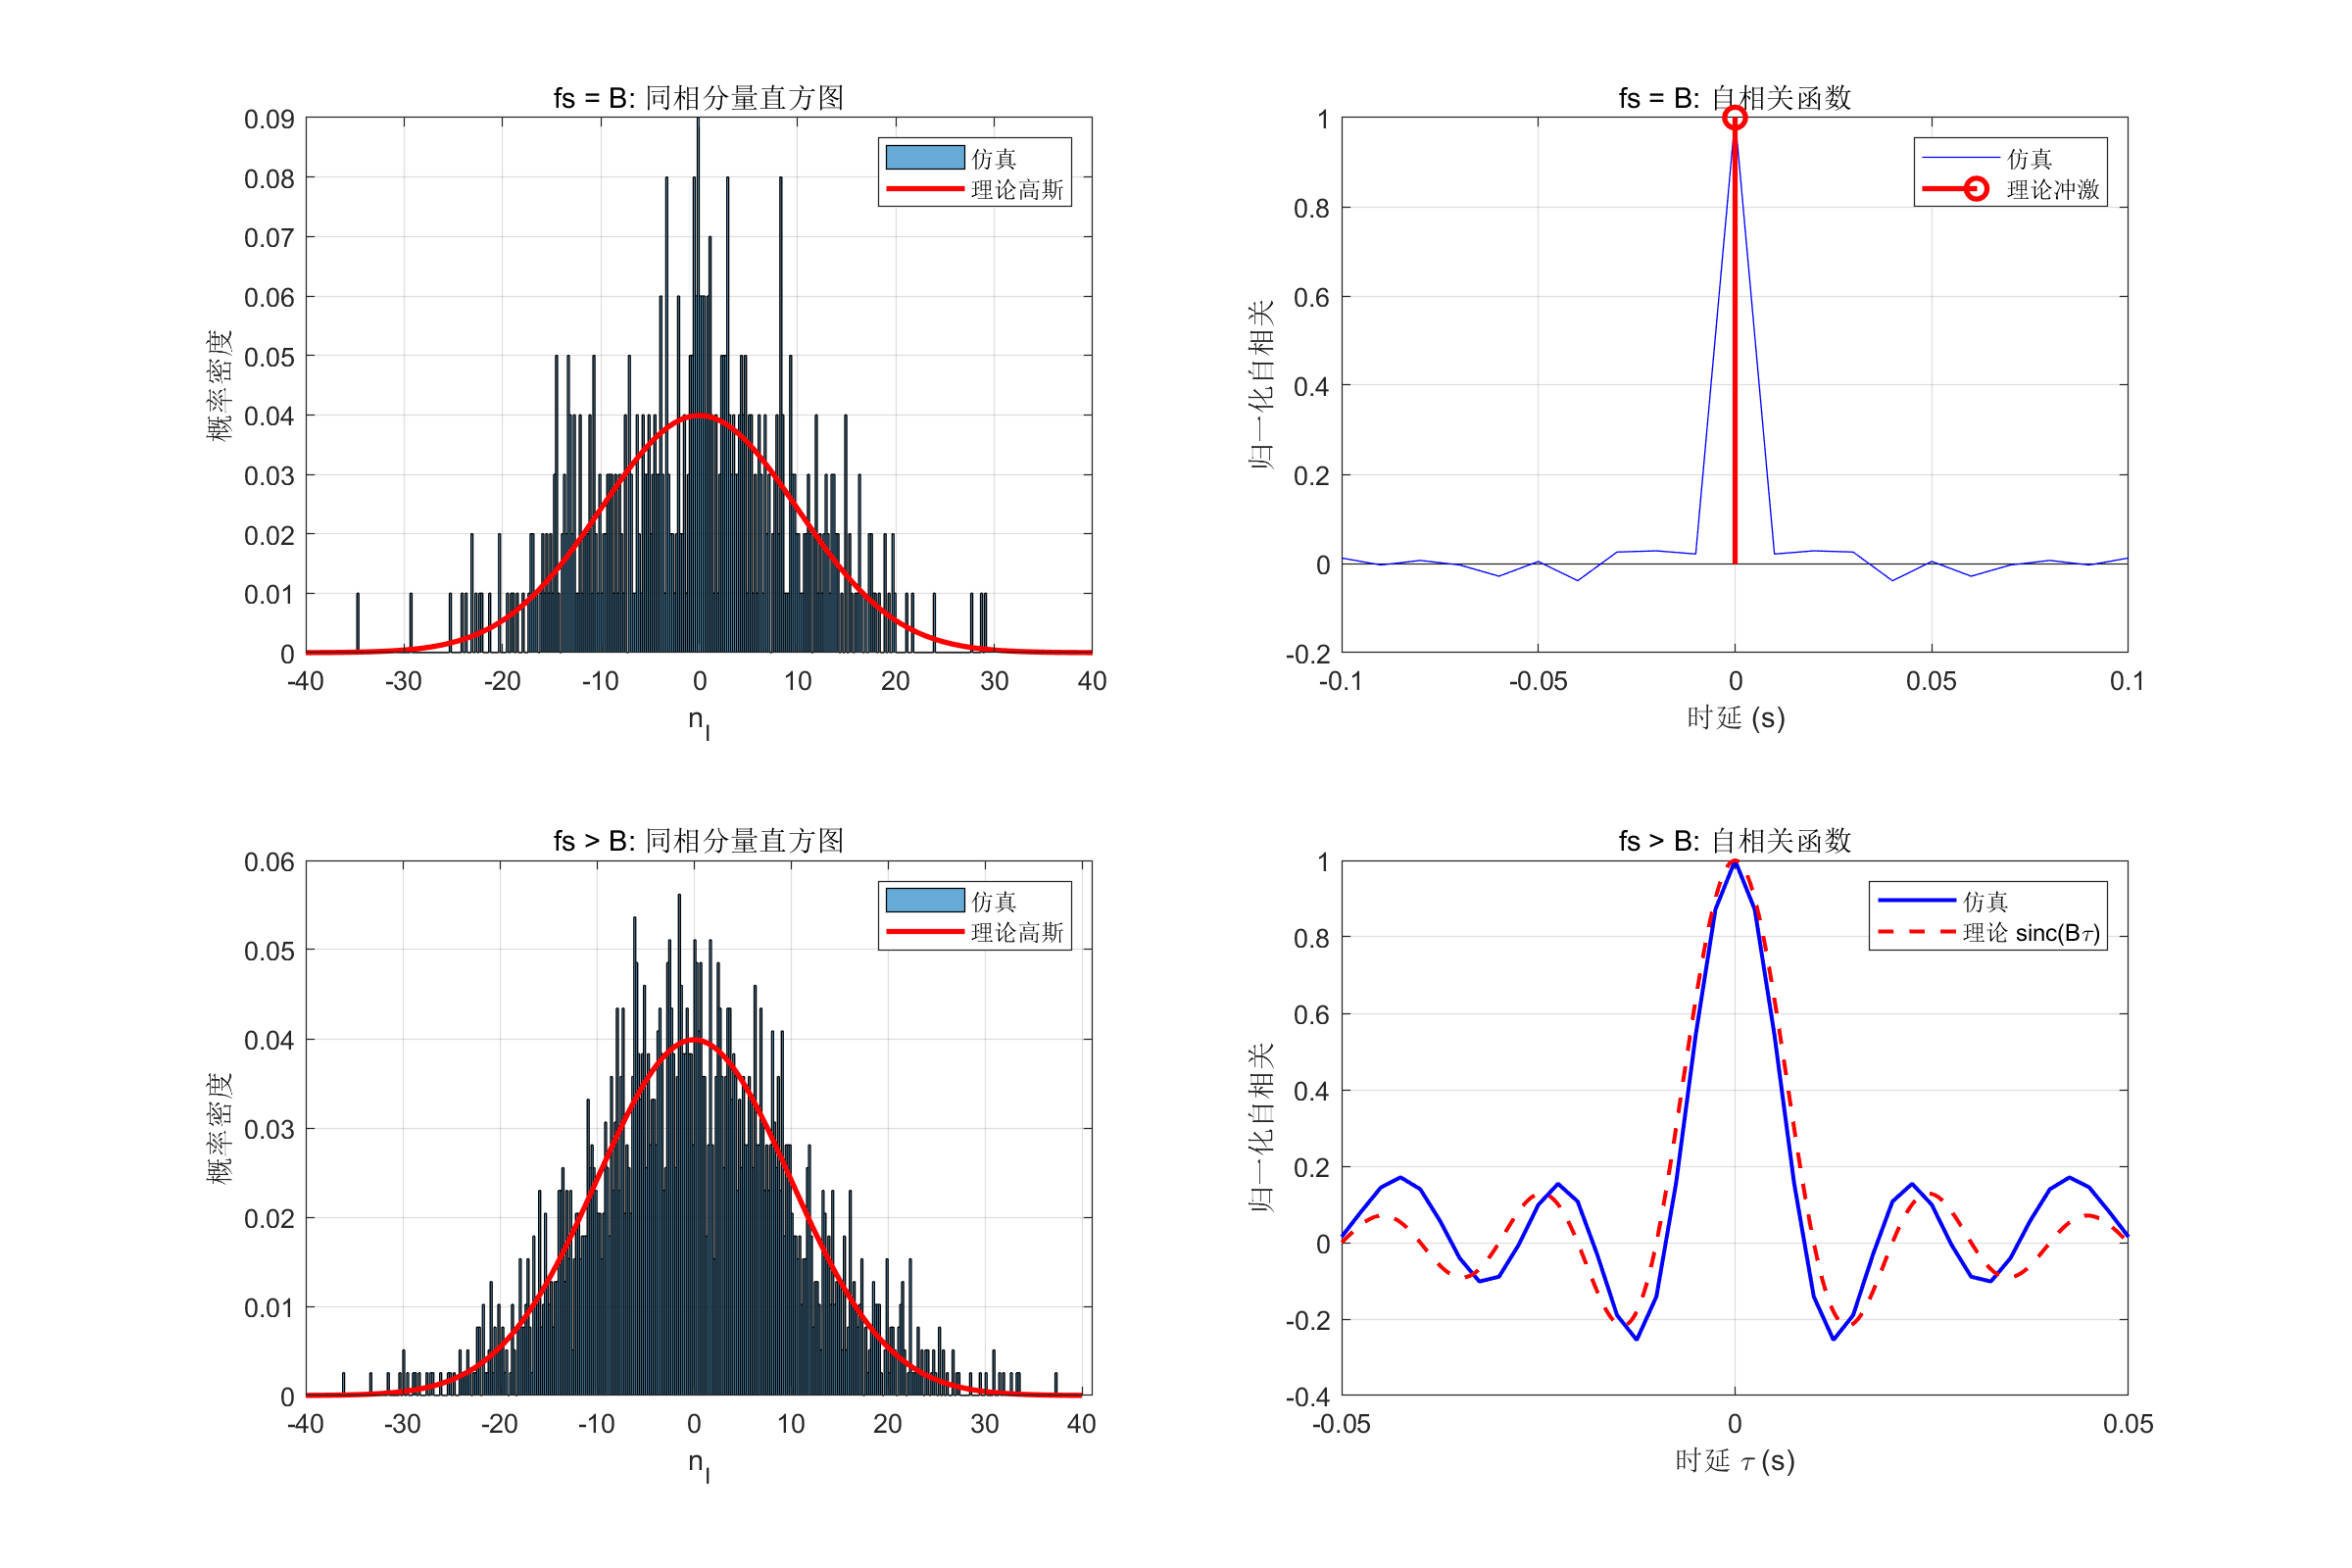
\includegraphics[width=\textwidth]{pdf_correlation}
    \caption{分布验证与自相关验证}
\end{figure}

\section{矩形基带信号}

生成长度为 \(L=10\) 的随机比特，映射为 \(\pm 1\) 符号，每个符号持续 \(T_s = 2/B\) 秒，通过重复每个符号得到矩形波形。采样率设置为每个符号100个样点。

代码如下（对应文件rect.m）：

\begin{lstlisting}[language = MATLAB]
clear; clc; close all;

%% 参数设置
B = 100;            % 带宽 (Hz)
Ts = 2/B;           % 符号周期
samples_per_symbol = 100;
fs = samples_per_symbol/Ts;        % 采样频率
L = 10;             % 矩形个数

%a_n的产生
bits = randi([0, 1], 1, L);   % 长度为 L 的随机比特
symbols = 2 * bits - 1; 

%矩形波的产生
m = repelem(symbols, samples_per_symbol);

t_total = L * Ts;                     % 总时长 (s)
t = linspace(0, t_total, length(m));  % 时间向量

figure;
plot(t, m, 'b-', 'LineWidth', 1.5);
xlabel('时间 (s)');
ylabel('幅度');
title('矩形基带信号 m(t)');
grid on;
ylim([-1.2, 1.2]);
\end{lstlisting}

仿真结果：

\begin{figure}[H]
    \centering
    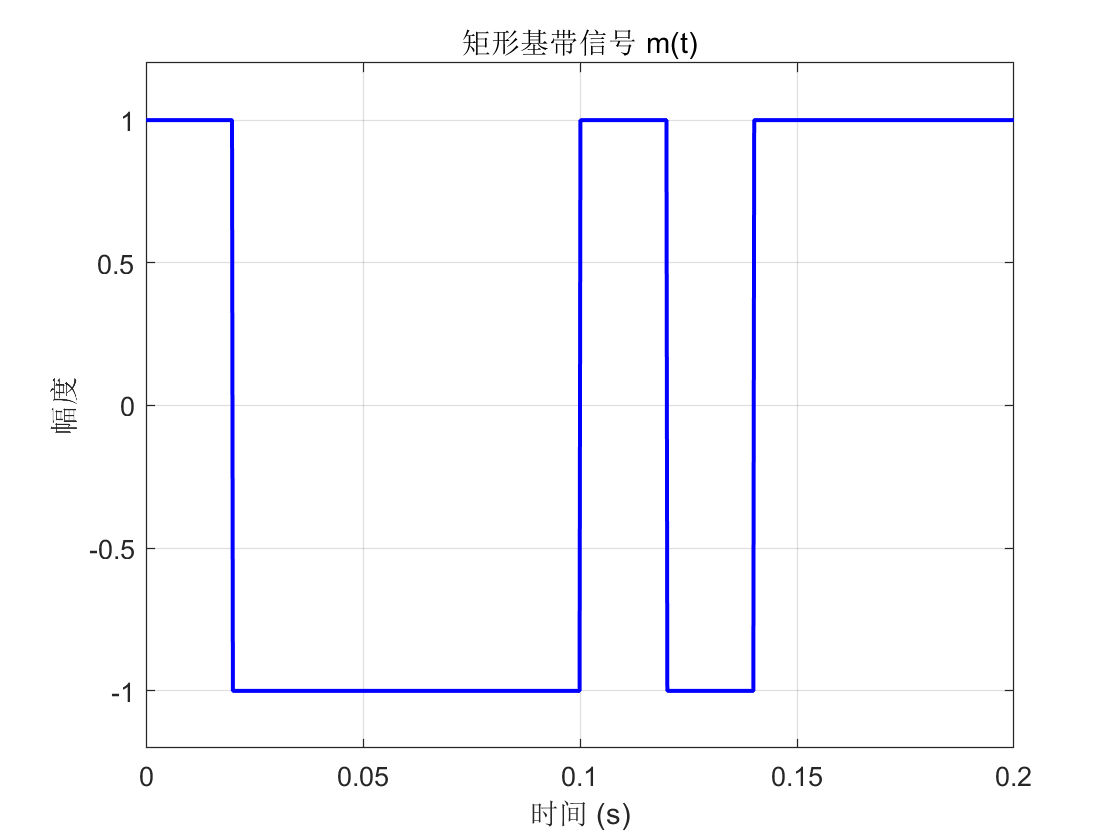
\includegraphics[width=0.6\textwidth]{rect.png}
    \caption{矩形基带信号}
\end{figure}

\section{DSB调制解调}

生成窄带高斯噪声和矩形基带信号，进行DSB调制（与载波相乘），加入噪声后进行相干解调（再次与载波相乘后低通滤波），得到解调输出 \(m(t)+n_c(t)\)。绘制窄带噪声同相分量、基带信号、已调信号和解调输出波形。

代码如下（对应文件  DSB.m）：

\begin{lstlisting}[language = MATLAB]
%参数设置
B = 100;        % 基波带宽(Hz)
fc = 1000;      % 载波频率(Hz)
samples_per_symbol = 2000;
fs = samples_per_symbol/Ts;        % 采样频率
L = 10;   

% 时间轴
t_total = L * Ts;               % 总时长
t = 0:1/fs:t_total-1/fs;        % 时间向量
Nsamples = length(t);           % 总采样点数

% 设定低通滤波器参数
f_cut = B/2;                % 低通滤波器截止频率 (Hz)
% 使用 fir1 设计等波纹 FIR 滤波器
filter_order = 200;         % 滤波器阶数
h_lp = fir1(filter_order, f_cut/(fs/2), 'low'); % 归一化截止频率

%噪声产生
N0 = 1e-5;
Pn = N0 * B;
white_noise = randn(1, Nsamples);
n_c_filt = filter(h_lp, 1, white_noise);
%计算实际功率，并调整到 Pn
actual_power = var(n_c_filt);
n_c = n_c_filt * sqrt(Pn / actual_power);
%正交分量
white_noise_q = randn(1, Nsamples);
n_s_filt = filter(h_lp, 1, white_noise_q);
actual_power_q = var(n_s_filt);
n_s = n_s_filt * sqrt(Pn / actual_power_q);

%矩形波
bits = randi([0, 1], 1, L);   % 长度为 L 的随机比特
symbols = 2 * bits - 1; 
m = repelem(symbols, samples_per_symbol);

%载波
carrier_cos = cos(2*pi*fc*t);
carrier_sin = sin(2*pi*fc*t);
s_t = m .* carrier_cos;                         % DSB调制
n_t = n_c .* carrier_cos - n_s .* carrier_sin;  % 窄带噪声
r_t = s_t + n_t;                                % 接收信号

%相干解调
demod = 2 * r_t .* carrier_cos;
n_t = n_c .* carrier_cos - n_s .* carrier_sin;
demod_out = filtfilt(h_lp, 1, demod);
% 由于滤波初始瞬态，丢弃前 filter_order 个样本
start_idx = filter_order + 1;
demod_out = demod_out(start_idx:end);
t_adj = t(start_idx:end);
m_adj = m(start_idx:end);
n_c_adj = n_c(start_idx:end);

%绘制波形
figure('Name', 'DSB调制与解调波形', 'Position', [100, 100, 1200, 800]);

% 子图1：窄带高斯噪声的同相分量 n_c(t)（局部，显示前 0.03 秒）
t_limit_nc = 0.03;  % 显示时间长度
idx_nc = t_adj <= t_limit_nc;
subplot(2,2,1);
plot(t_adj(idx_nc), n_c_adj(idx_nc), 'b', 'LineWidth', 1);
xlabel('时间 (s)'); ylabel('幅度');
title('窄带高斯噪声同相分量 n_c(t)');
grid on;

% 子图2：DSB 同相分量 = 基带信号 m(t)
subplot(2,2,2);
plot(t, m, 'b-', 'LineWidth', 1.5);
xlabel('时间 (s)');
ylabel('幅度');
title('矩形基带信号 m(t)');
grid on;
ylim([-1.2, 1.2]);

% 子图3：DSB 已调信号 s(t)
idx_s = t <= Ts;
subplot(2,2,3);
plot(t(idx_s), s_t(idx_s), 'g', 'LineWidth', 1);
xlabel('时间 (s)'); ylabel('幅度');
title('DSB 已调信号 s(t)');
grid on;

% 子图4：DSB 相干解调输出
idx_full = t_adj <= t_total;

subplot(2,2,4);
plot(t_adj(idx_full), m_adj(idx_full), 'r--', 'LineWidth', 1.2); hold on;
plot(t_adj(idx_full), demod_out(idx_full), 'b-', 'LineWidth', 1);
xlabel('时间 (s)'); ylabel('幅度');
title('DSB 相干解调输出');
legend('原始 m(t)', '解调输出 m(t)+n_c(t)', 'Location', 'best');
grid on;
ylim([-2, 2]);
hold off;

sgtitle('DSB 调制与解调实验波形');
\end{lstlisting}

仿真结果：

\begin{figure}[H]
    \centering
    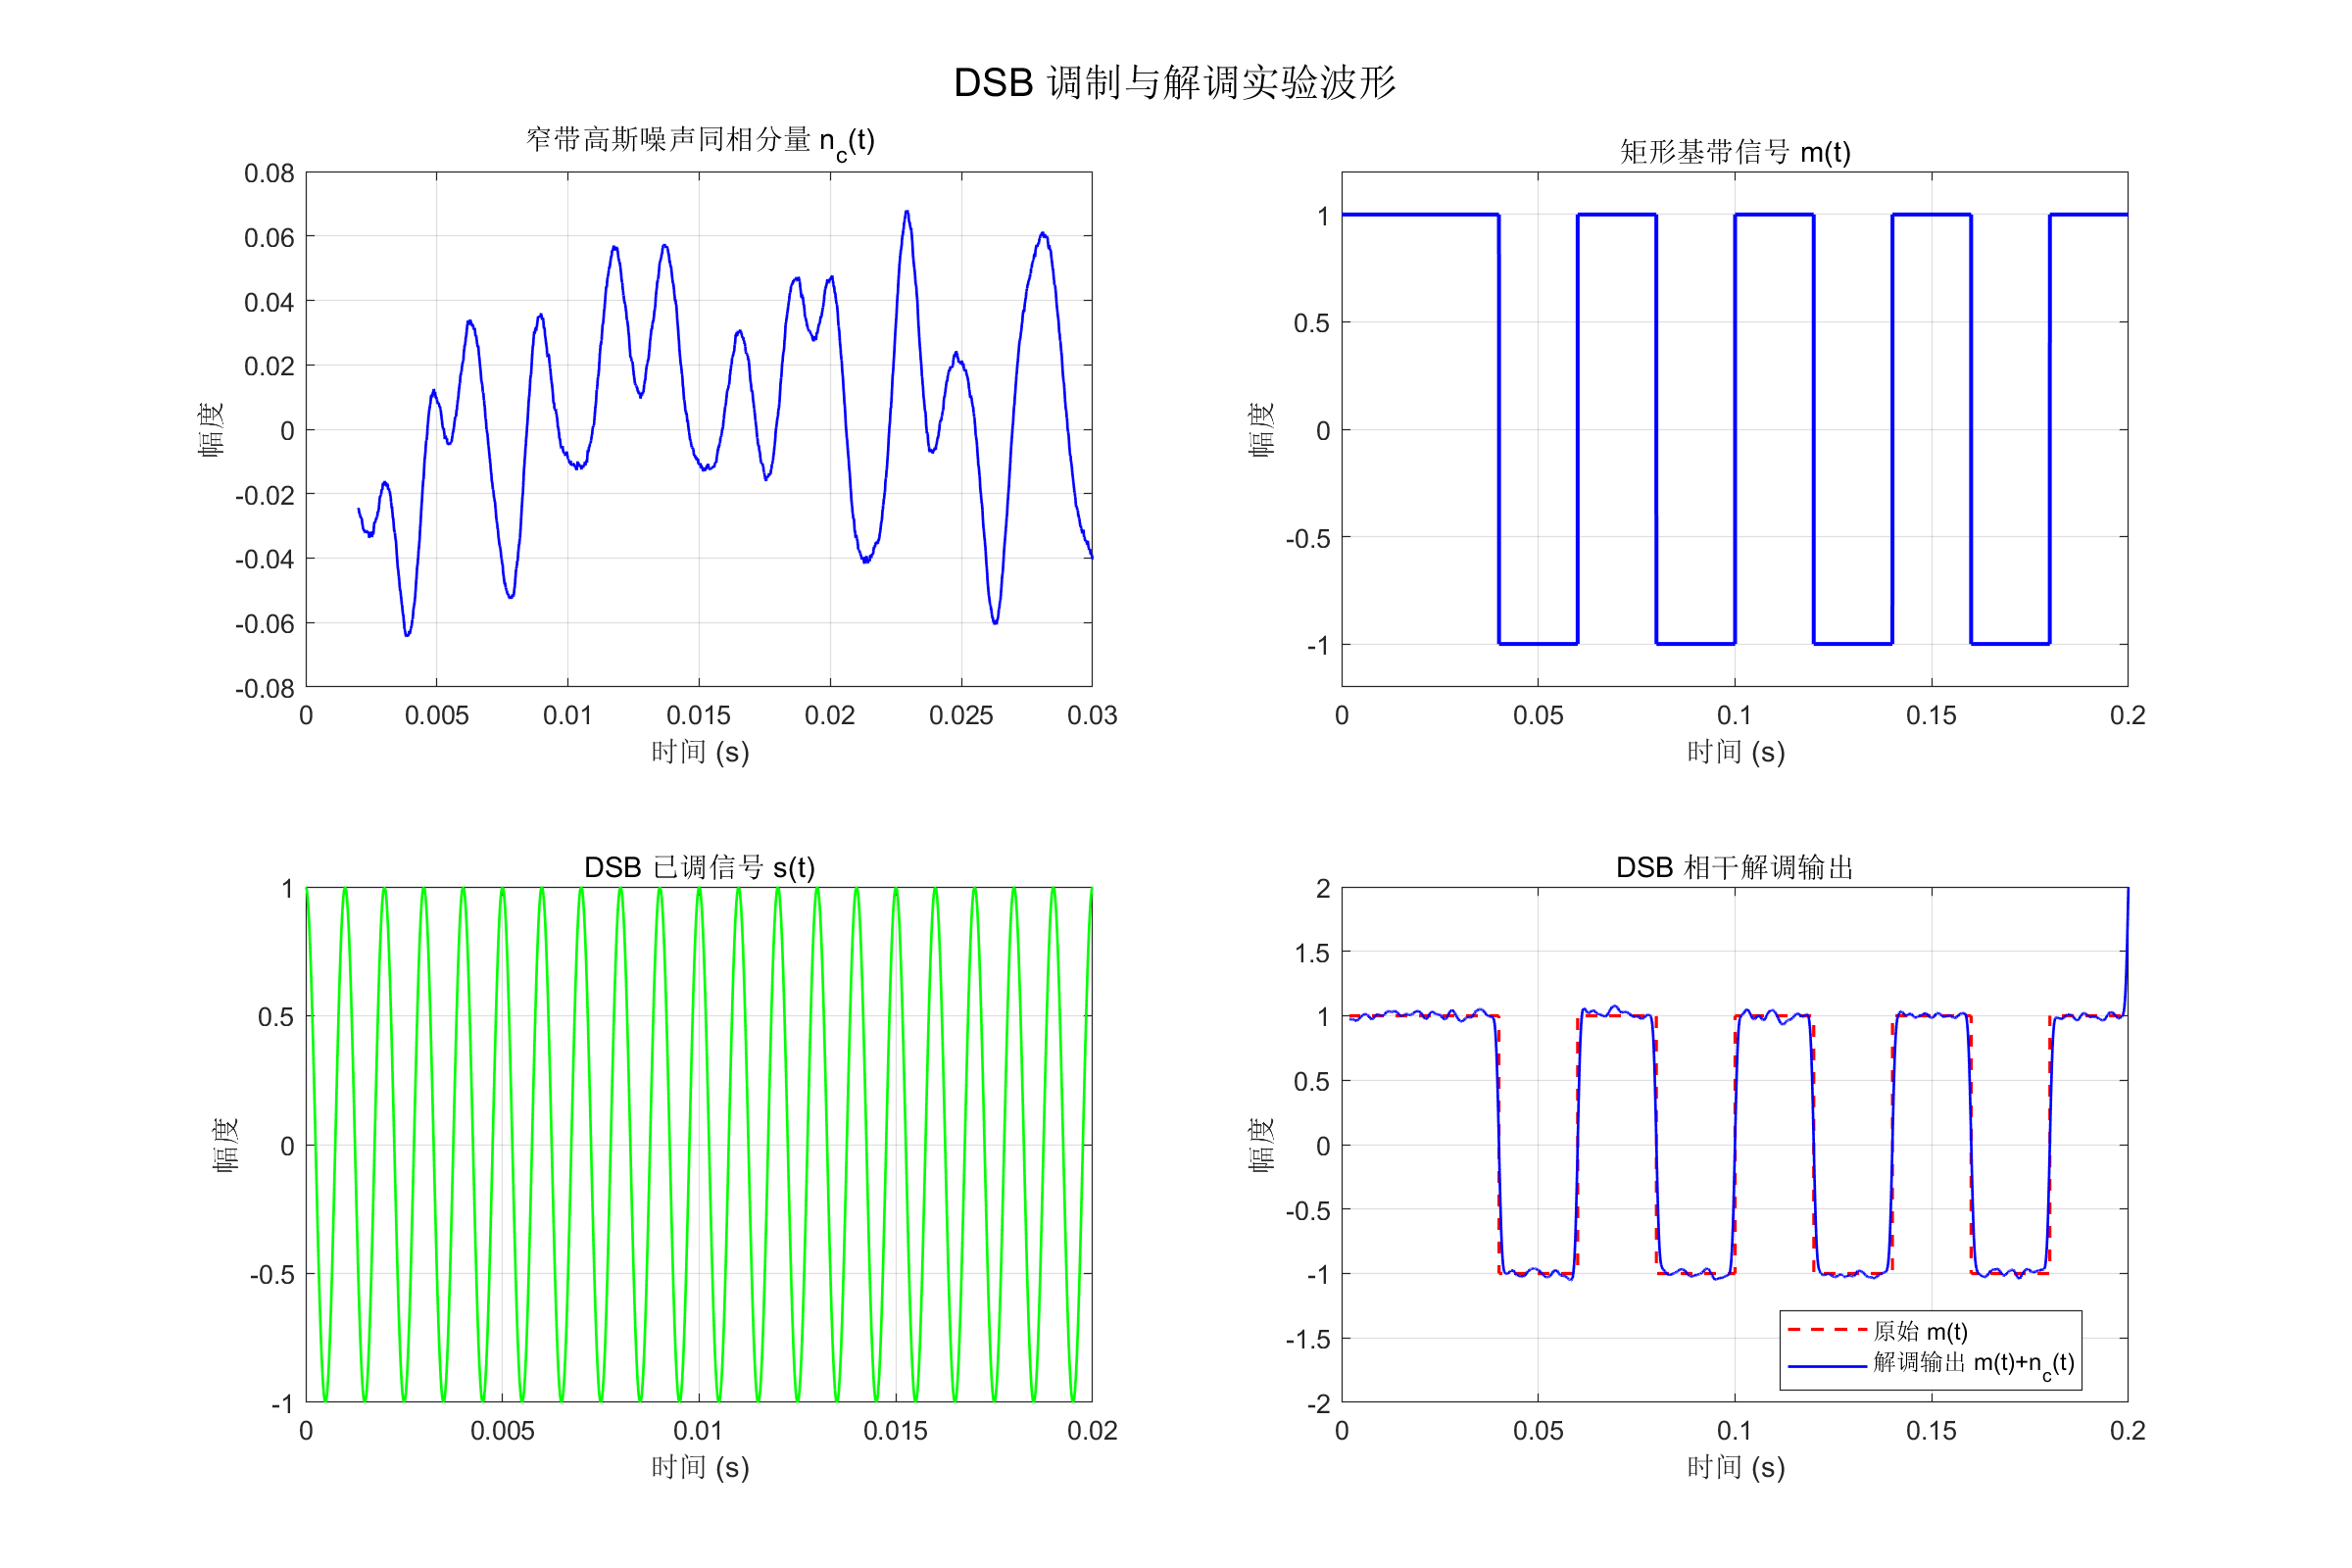
\includegraphics[width=\textwidth]{DSB.png}
    \caption{DSB调制解调(1)}
\end{figure}

\begin{figure}[H]
    \centering
    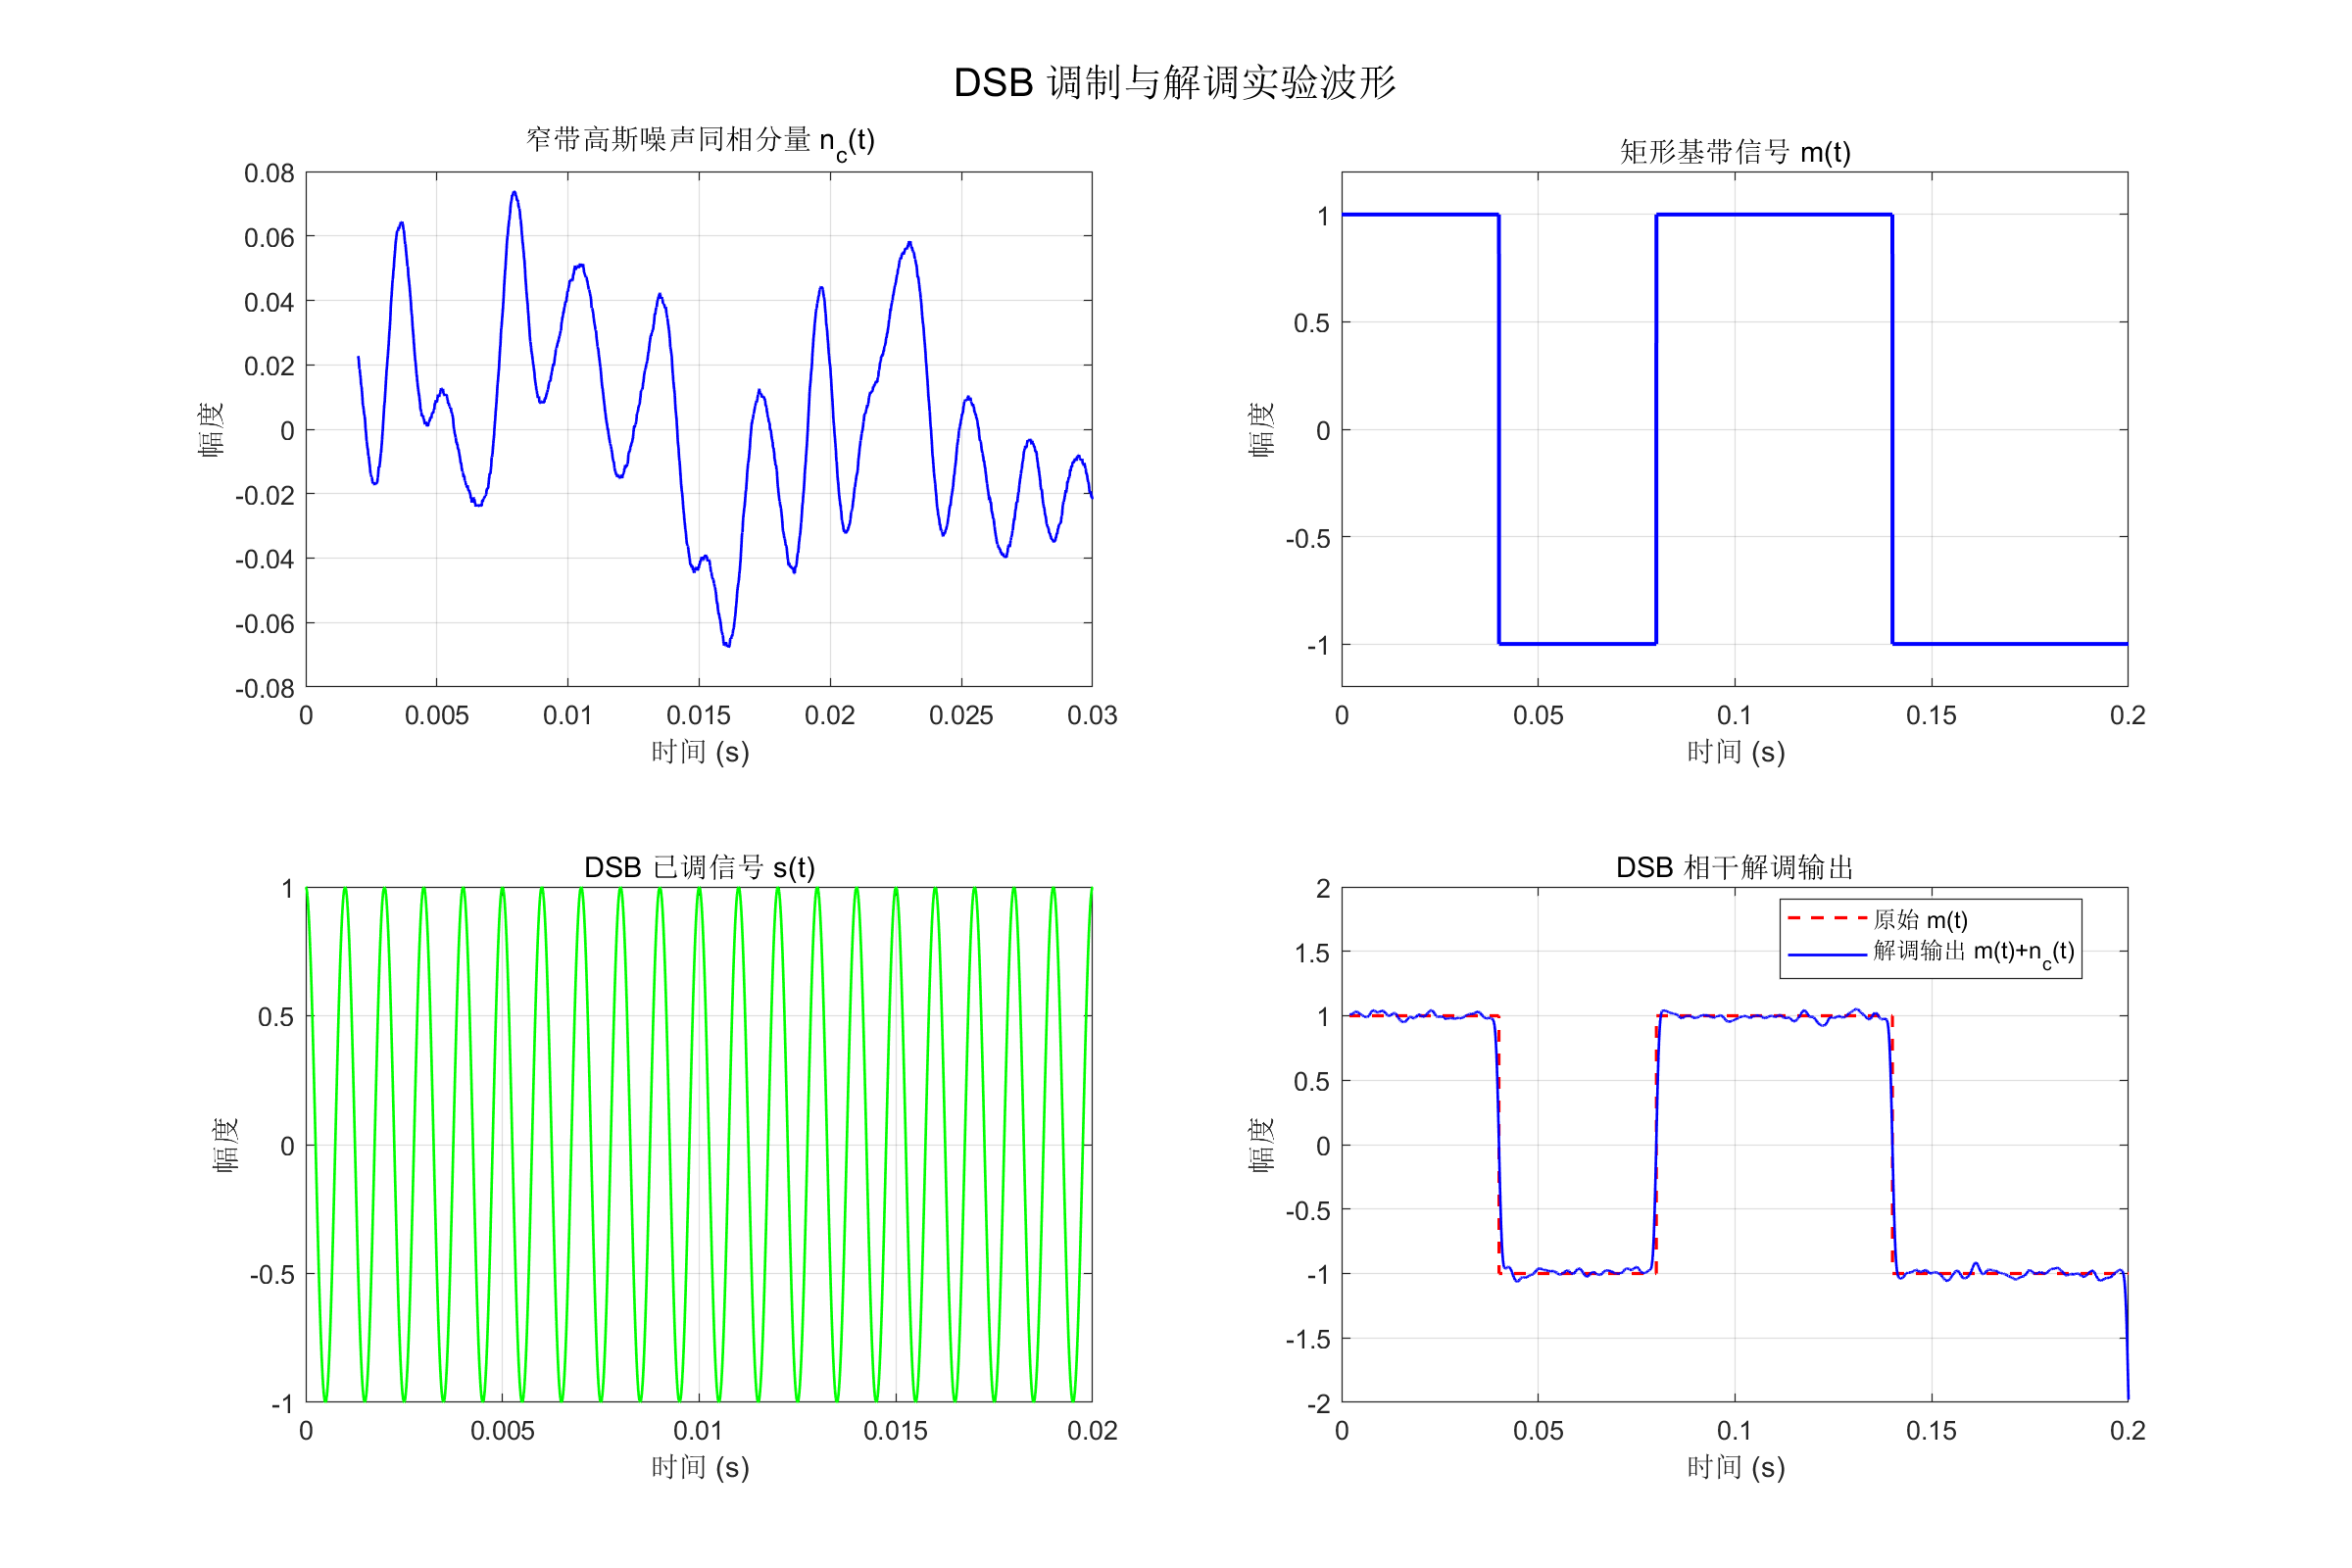
\includegraphics[width=\textwidth]{DSB1.png}
    \caption{DSB调制解调(2)}
\end{figure}

\section{AM调制解调}

AM调制信号为 \(s(t)=[1+am(t)]\cos 2\pi f_c t\)，其中调制指数 \(a=0.8\)。相干解调后需去除直流分量得到 \(a m(t)+n_c(t)\)。绘制窄带噪声同相分量、基带信号、AM同向分量、已调信号和解调输出波形。

代码如下（对应文件AM.m）：

\begin{lstlisting}[language = MATLAB]
clear; clc; close all;

%% 参数设置
B = 100;                    % 基带信号带宽 (Hz)
fc = 1000;                  % 载波频率 (Hz)
Ts = 1 / B;                 % 符号周期 (s)
samples_per_symbol = 2000;
fs = samples_per_symbol / Ts;   % 采样频率 (Hz)
L = 10;                     % 符号个数

t_total = L * Ts;           % 总时长 = 0.1 s
t = 0 : 1/fs : t_total - 1/fs;
Nsamples = length(t);

a = 0.8;                    % 调制指数

% 窄带噪声参数
N0 = 1e-4;                  % 双边带功率谱密度 (W/Hz)
Pn_c = N0 * B / 2;          % 同相分量 n_c(t) 的功率

% 低通滤波器设计
f_cut = B / 2;              % 低通截止频率 (Hz)
filter_order = 200;         % 滤波器阶数
h_lp = fir1(filter_order, f_cut/(fs/2), 'low');

%% 生成窄带高斯噪声的同相分量和正交分量
n_c_filt = filter(h_lp, 1, randn(1, Nsamples));
actual_power_c = var(n_c_filt);
n_c = n_c_filt * sqrt(Pn_c / actual_power_c);

n_s_filt = filter(h_lp, 1, randn(1, Nsamples));
actual_power_s = var(n_s_filt);
n_s = n_s_filt * sqrt(Pn_c / actual_power_s);

% 载波
carrier_cos = cos(2*pi*fc*t);
carrier_sin = sin(2*pi*fc*t);

n_t = n_c .* carrier_cos - n_s .* carrier_sin;

%% 基带信号调制解调
bits = randi([0, 1], 1, L);
symbols = 2*bits - 1;
m = repelem(symbols, samples_per_symbol);

s_t = (1 + a * m) .* carrier_cos;

r_t = s_t + n_t;

demod = 2 * r_t .* carrier_cos;
demod_filt = filtfilt(h_lp, 1, demod);

% 滤除滤波器初始瞬态
start_idx = filter_order + 1;
t_adj = t(start_idx:end);
m_adj = m(start_idx:end);
n_c_adj = n_c(start_idx:end);
demod_out = demod_filt(start_idx:end);

demod_ac = demod_out - mean(demod_out);
am_theory_ac = a * m_adj;

%% 绘图
figure('Name', 'AM 调制与解调实验', 'Position', [100, 100, 1200, 800]);

% 子图1：窄带高斯噪声同相分量 n_c(t)
t_limit_noise = 0.03;
idx_noise = t_adj <= t_limit_noise;
subplot(2,3,1);
plot(t_adj(idx_noise), n_c_adj(idx_noise), 'b', 'LineWidth', 1);
xlabel('时间 (s)'); ylabel('幅度');
title('窄带高斯噪声同相分量 n_c(t)');
grid on;

% 子图2：基带信号 m(t)
subplot(2,3,2);
plot(t, m, 'r', 'LineWidth', 1.2);
xlabel('时间 (s)'); ylabel('幅度');
title('矩形基带信号 m(t)');
grid on;
ylim([-1.2, 1.2]);

% 子图3：AM 同向分量 = 1 + a*m(t)
subplot(2,3,3);
am_envelope = 1 + a * m;
plot(t, am_envelope, 'm', 'LineWidth', 1.2);
xlabel('时间 (s)'); ylabel('幅度');
title('AM 同向分量 1 + a·m(t)');
grid on;
ylim([-0.2, 2.2]);

% 子图4：AM 已调信号 s(t)
t_carrier_limit = 5 / fc;      % 5 个载波周期
idx_s = t <= t_carrier_limit;
subplot(2,3,4);
plot(t(idx_s), s_t(idx_s), 'g', 'LineWidth', 1);
xlabel('时间 (s)'); ylabel('幅度');
title('AM 已调信号 s(t)');
grid on;

% 子图5：AM 相干解调输出
subplot(2,3,5);
plot(t_adj, am_theory_ac, 'r--', 'LineWidth', 1.2); hold on;
plot(t_adj, demod_ac, 'b', 'LineWidth', 1);
xlabel('时间 (s)'); ylabel('幅度');
title('AM 相干解调输出（去直流）');
legend('理论 a·m(t)', '解调输出 a·m(t)+n_c(t)', 'Location', 'best');
grid on;
ylim([-1.5, 1.5]);
hold off;

% 子图6：留空
subplot(2,3,6);
axis off;

sgtitle('AM 调制与解调实验波形', 'FontSize', 14);
tight;
\end{lstlisting}

\begin{figure}[H]
    \centering
    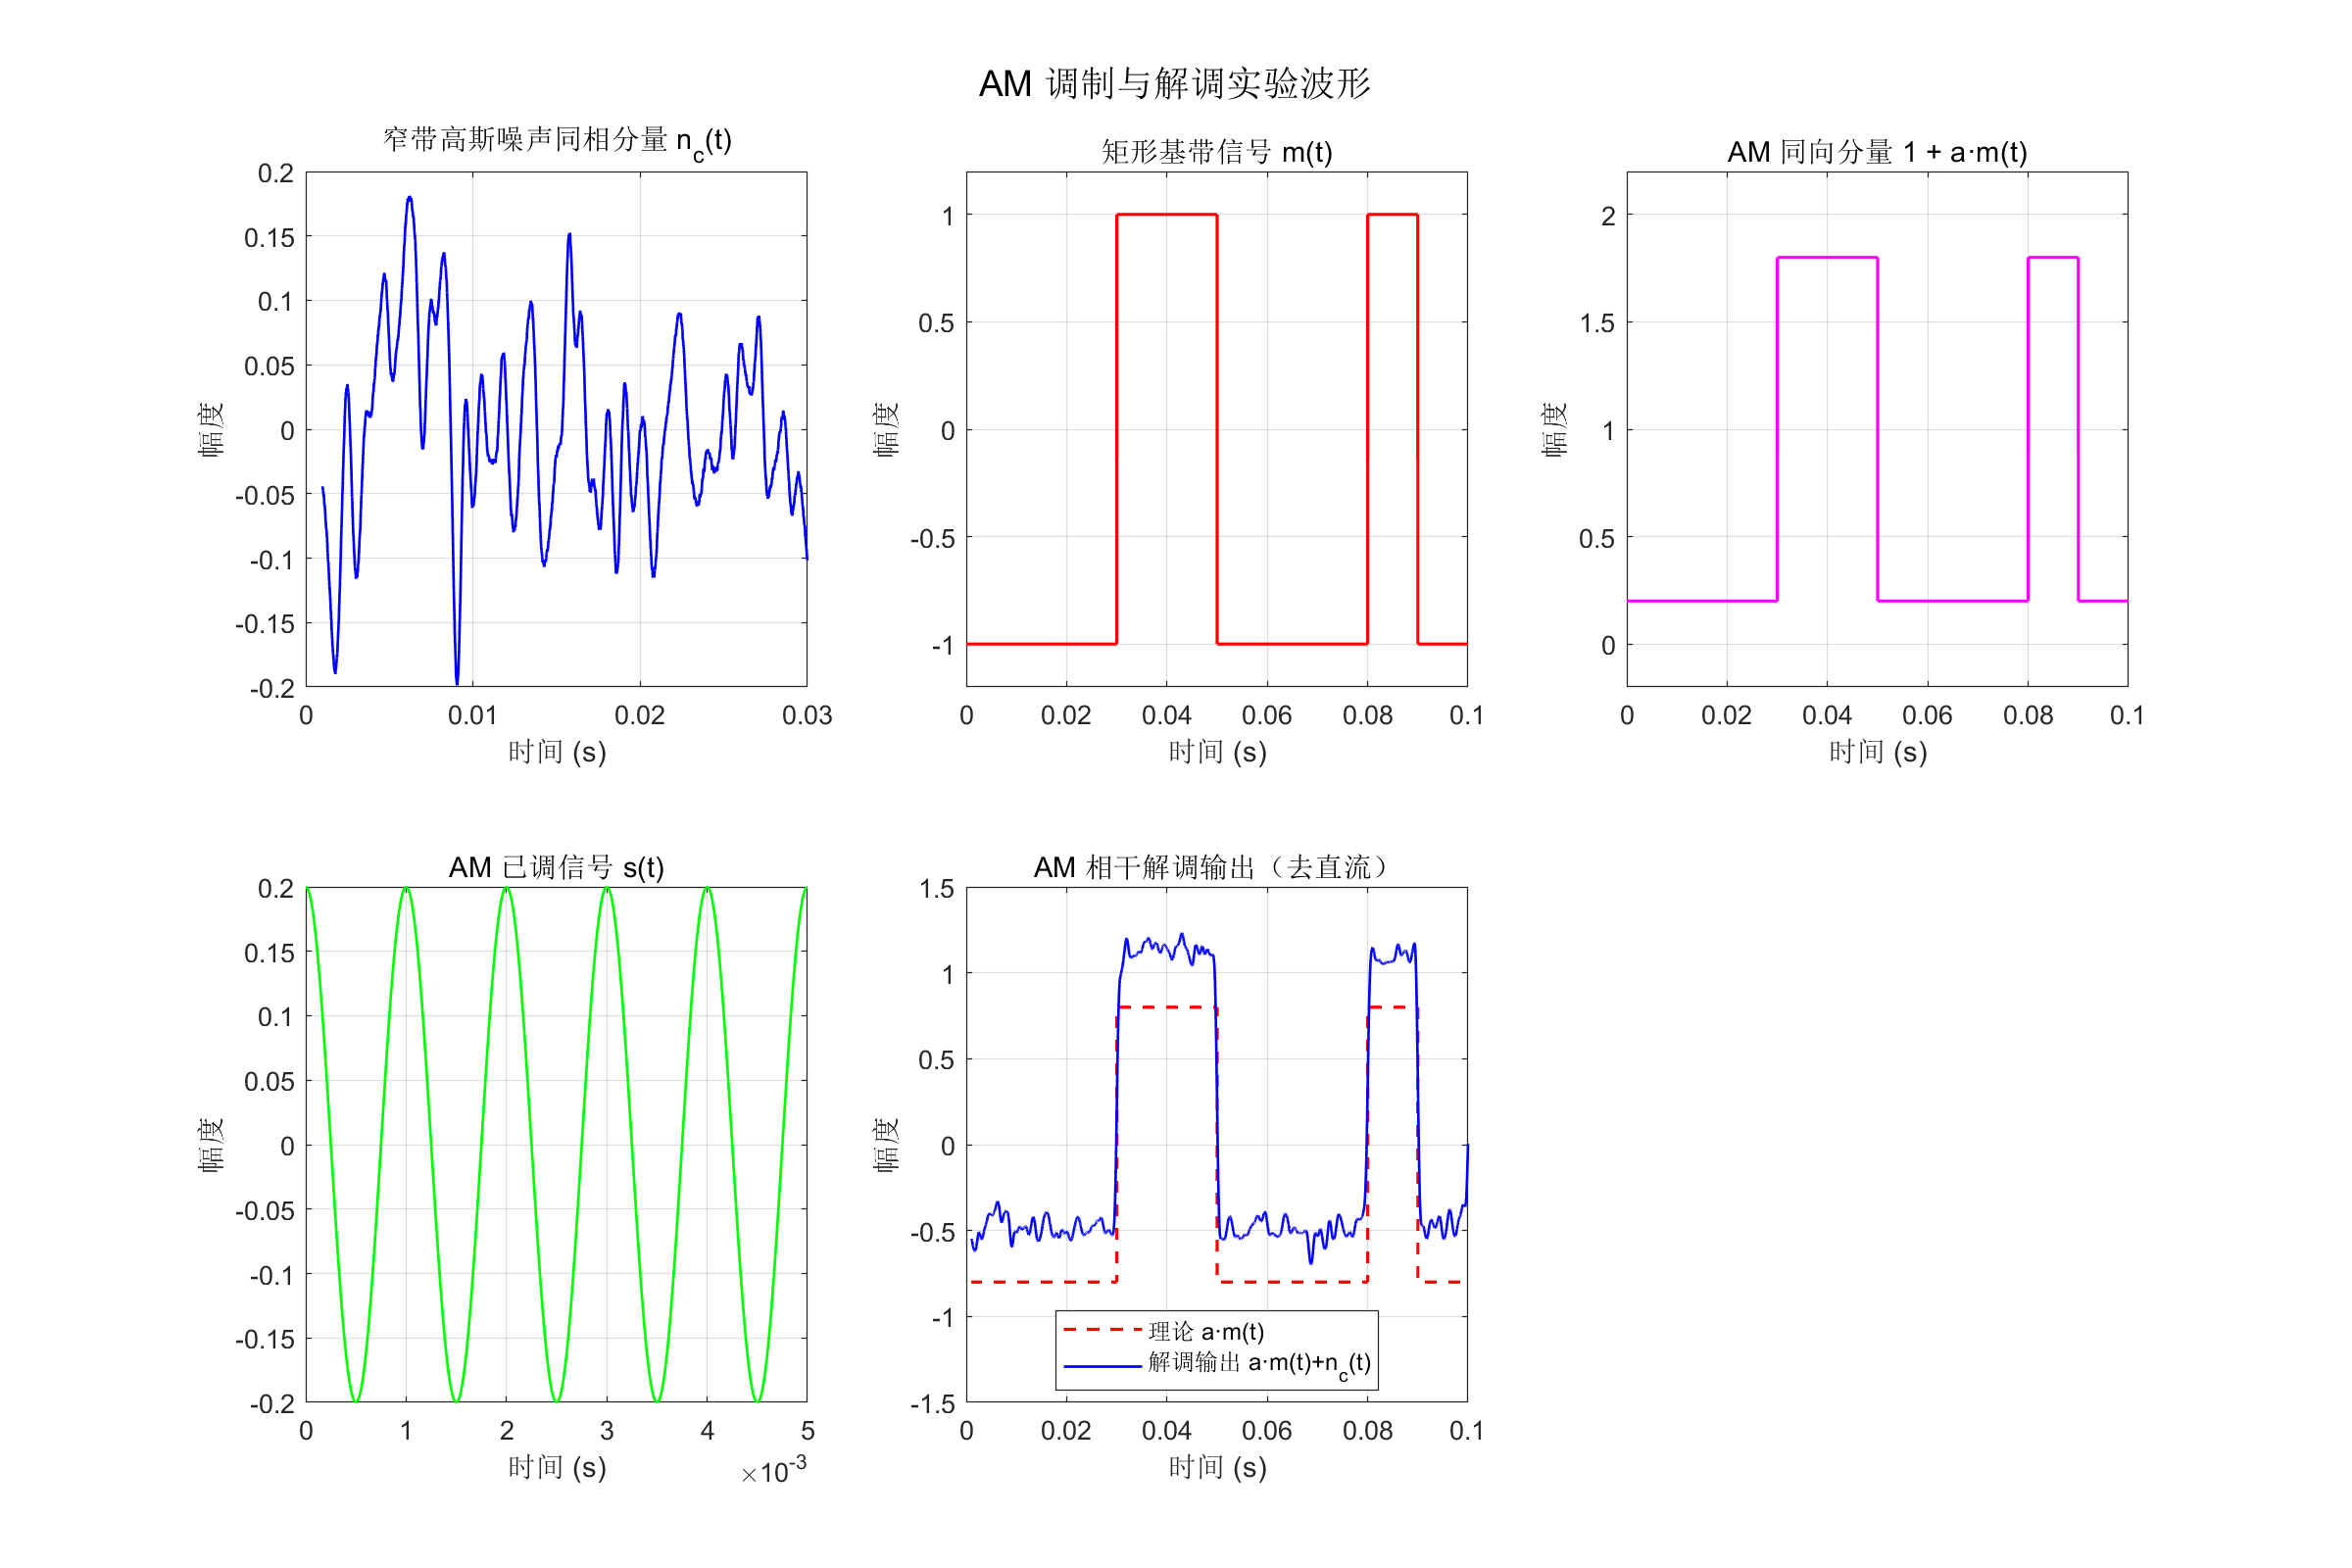
\includegraphics[width = \textwidth]{AM.png}
    \caption{AM调制解调波形}
\end{figure}

\end{document}